\documentclass[a4paper,12pt]{article}

\usepackage{graphicx}
\usepackage{listings}
\usepackage{xcolor}
\usepackage{titlesec}
\usepackage{setspace}
\usepackage{caption}
\usepackage{float}

\graphicspath{ {./images/} }

\lstset{
  basicstyle=\ttfamily\footnotesize,
  breaklines=true,
  breakatwhitespace=true,
  columns=fullflexible,
  frame=single,
  backgroundcolor=\color[RGB]{248,248,248},
  keywordstyle=\color{blue},
  commentstyle=\color{gray},
  stringstyle=\color{orange},
  showstringspaces=false
}

\makeatletter
\def\maketitle{
  \begin{titlepage}
    \centering
    \vspace*{-1cm}
    
\includegraphics[width=0.5\textwidth]{yu-logo.png}\\[2cm]
    {\huge\bfseries Using jSparrow: Our Experience and Insights}\\[2cm]
    {\Large College of Engineering and Architecture}\\
    {Al-Yamamah University}\\
    {Kingdom of Saudi Arabia, Riyadh}\\[1cm]
    SWE 402: Software Maintenance and Evolution\\[2cm]
    {\large\bfseries Prepared By:}\\[0.3cm]
    YAZED ALKHALAF - 202211123\\
    SAIMAN TAKLAS - 202021400\\
    ALI BA WAZIR  - 202211018\\
    [2cm]
    {\large\bfseries Submitted To:}\\[0.3cm]
    Dr. Khaled Makhadmeh\\[2cm]
    {\large \today}
    \vfill
  \end{titlepage}
}
\makeatother

\begin{document}

\maketitle

\section{Introduction}

jSparrow is a refactoring tool for Java that automates the identification and resolution of code smells, aiming to improve the structure, performance, and maintainability of software. In this project, we document our experience using the free version of jSparrow to refactor a sample Java codebase of approximately 100 lines. The objective was to test how well the tool handles various common bad smells that were deliberately injected into our code.

\section{The Test Subject}

We created a basic student management system containing multiple common Java bad smells such as redundant semicolons, improper use of string equality, unused imports, and poor enum handling. The original version of the test code is shown in \textbf{Listing~\ref{lst:test-subject}}.

\begin{lstlisting}[language=Java, caption={Original Test Subject Java Code}, label={lst:test-subject}]
  package main;

  import java.util.ArrayList;
  import java.util.Scanner;
  import java.util.Random; // unused
  import java.util.Hashtable; // unused
  
  public class StudentManagementSystem {
      ArrayList<String> studentNames = new ArrayList<>(); ArrayList<Integer> studentIds = new ArrayList<>(); ArrayList<Double> studentGPAs = new ArrayList<>();;
  
      public void menu() {
          Scanner scanner = new Scanner(System.in);
          while (true) {
              System.out.println("1. Add");
              System.out.println("2. Show");
              System.out.println("3. Find");
              System.out.println("4. Exit");
              int opt = scanner.nextInt(); scanner.nextLine();
              if (opt == 1) {
                  add(scanner);
              } else {
                  if (opt == 2) {
                      show();
                  } else {
                      if (opt == 3) {
                          find(scanner);
                      } else {
                          if (opt == 4) {
                              System.out.println("Bye"); break;
                          } else {
                              System.out.println("Wrong");
                          }
                      }
                  }
              }
          }
          scanner.close();
      }
  
      void add(Scanner scanner) {
          System.out.println("Name?");
          String name = scanner.nextLine();
          System.out.println("ID?");
          int id = scanner.nextInt(); scanner.nextLine();
          System.out.println("GPA?");
          double gpa = scanner.nextDouble(); scanner.nextLine();
  
          studentNames.add(name);
          studentIds.add(id);
          studentGPAs.add(gpa);
  
          System.out.println("Added");
      }
  
      void show() {
          for (int i = 0; i < studentNames.size(); i++) {
              if (!(studentNames.get(i) == null)) {
                  if (studentNames.get(i).toString().equals("")) {
                      System.out.println("Empty name");
                  } else {
                      System.out.println("Name: " + studentNames.get(i));
                  }
              }
              System.out.println("ID: " + studentIds.get(i));
              System.out.println("GPA: " + studentGPAs.get(i));;
          }
      }
  
      void find(Scanner scanner) throws IllegalArgumentException {
          System.out.println("Search name:");
          String q = scanner.nextLine();
          if (q == null || q.equals("")) {
              throw new IllegalArgumentException("Bad input");
          }
  
          boolean found = false;
          for (int i = 0; i < studentNames.size(); i++) {
              if (studentNames.get(i).equalsIgnoreCase(q)) {
                  System.out.println("Found: " + studentNames.get(i) + ", ID: " + studentIds.get(i));
                  found = true;
                  break;
              }
          }
  
          if (!found) {
              System.out.println("Not found");
          }
      }
  
      void deadMethod1() {
          String a = "useless";
          String b = "code";
          System.out.println(a + b); // never called
      }
  
      void messyEnums(Color c) {
          if (c.equals(Color.RED)) {
              System.out.println("Red");
          } else if (c.equals(Color.GREEN)) {
              System.out.println("Green");
          } else if (c.equals(Color.BLUE)) {
              System.out.println("Blue");
          }
      }
  
      public static void main(String[] args) {
          StudentManagementSystem s = new StudentManagementSystem(); s.menu();
      }
  
      enum Color {
          RED, GREEN, BLUE
      }
  }  
\end{lstlisting}

\newpage 

\section{Refactored Code by jSparrow}

After running jSparrow, we obtained the refactored version of the same program. The transformed version is shown in \textbf{Listing~\ref{lst:jsparrow-result}}.

\begin{lstlisting}[language=Java, caption={Refactored Code Generated by jSparrow}, label={lst:jsparrow-result}]
  package main;

  import java.util.ArrayList;
  import java.util.Scanner;
  
  public class StudentManagementSystem {
      ArrayList<String> studentNames = new ArrayList<>(); ArrayList<Integer> studentIds = new ArrayList<>(); ArrayList<Double> studentGPAs = new ArrayList<>();;
  
      public void menu() {
          Scanner scanner = new Scanner(System.in);
          while (true) {
              System.out.println("1. Add");
              System.out.println("2. Show");
              System.out.println("3. Find");
              System.out.println("4. Exit");
              int opt = scanner.nextInt(); scanner.nextLine();
              if (opt == 1) {
                  add(scanner);
              } else {
                  if (opt == 2) {
                      show();
                  } else {
                      if (opt == 3) {
                          find(scanner);
                      } else {
                          if (opt == 4) {
                              System.out.println("Bye"); break;
                          } else {
                              System.out.println("Wrong");
                          }
                      }
                  }
              }
          }
          scanner.close();
      }
  
      void add(Scanner scanner) {
          System.out.println("Name?");
          String name = scanner.nextLine();
          System.out.println("ID?");
          int id = scanner.nextInt(); scanner.nextLine();
          System.out.println("GPA?");
          double gpa = scanner.nextDouble(); scanner.nextLine();
  
          studentNames.add(name);
          studentIds.add(id);
          studentGPAs.add(gpa);
  
          System.out.println("Added");
      }
  
      void show() {
          for (int i = 0; i < studentNames.size(); i++) {
              if (!(studentNames.get(i) == null)) {
                  if ("".equals(studentNames.get(i))) {
                      System.out.println("Empty name");
                  } else {
                      System.out.println("Name: " + studentNames.get(i));
                  }
              }
              System.out.println("ID: " + studentIds.get(i));
              System.out.println("GPA: " + studentGPAs.get(i));
          }
      }
  
      void find(Scanner scanner) {
          System.out.println("Search name:");
          String q = scanner.nextLine();
          if (q == null || "".equals(q)) {
              throw new IllegalArgumentException("Bad input");
          }
  
          boolean found = false;
          for (int i = 0; i < studentNames.size(); i++) {
              if (studentNames.get(i).equalsIgnoreCase(q)) {
                  System.out.println("Found: " + studentNames.get(i) + ", ID: " + studentIds.get(i));
                  found = true;
                  break;
              }
          }
  
          if (!found) {
              System.out.println("Not found");
          }
      }
  
      void deadMethod1() {
          String a = "useless";
          String b = "code";
          System.out.println(a + b); // never called
      }
  
      void messyEnums(Color c) {
          if (c == Color.RED) {
              System.out.println("Red");
          } else if (c == Color.GREEN) {
              System.out.println("Green");
          } else if (c == Color.BLUE) {
              System.out.println("Blue");
          }
      }
  
      public static void main(String[] args) {
          StudentManagementSystem s = new StudentManagementSystem(); s.menu();
      }
  
      enum Color {
          RED, GREEN, BLUE
      }
  }  
\end{lstlisting}

\section{Analysis of Refactoring Rules}

In this section, we analyze the impact of each rule applied by jSparrow using its visual interface. The images highlight the original code on the left and the refactored version on the right.

\begin{figure}[H]
  \centering
  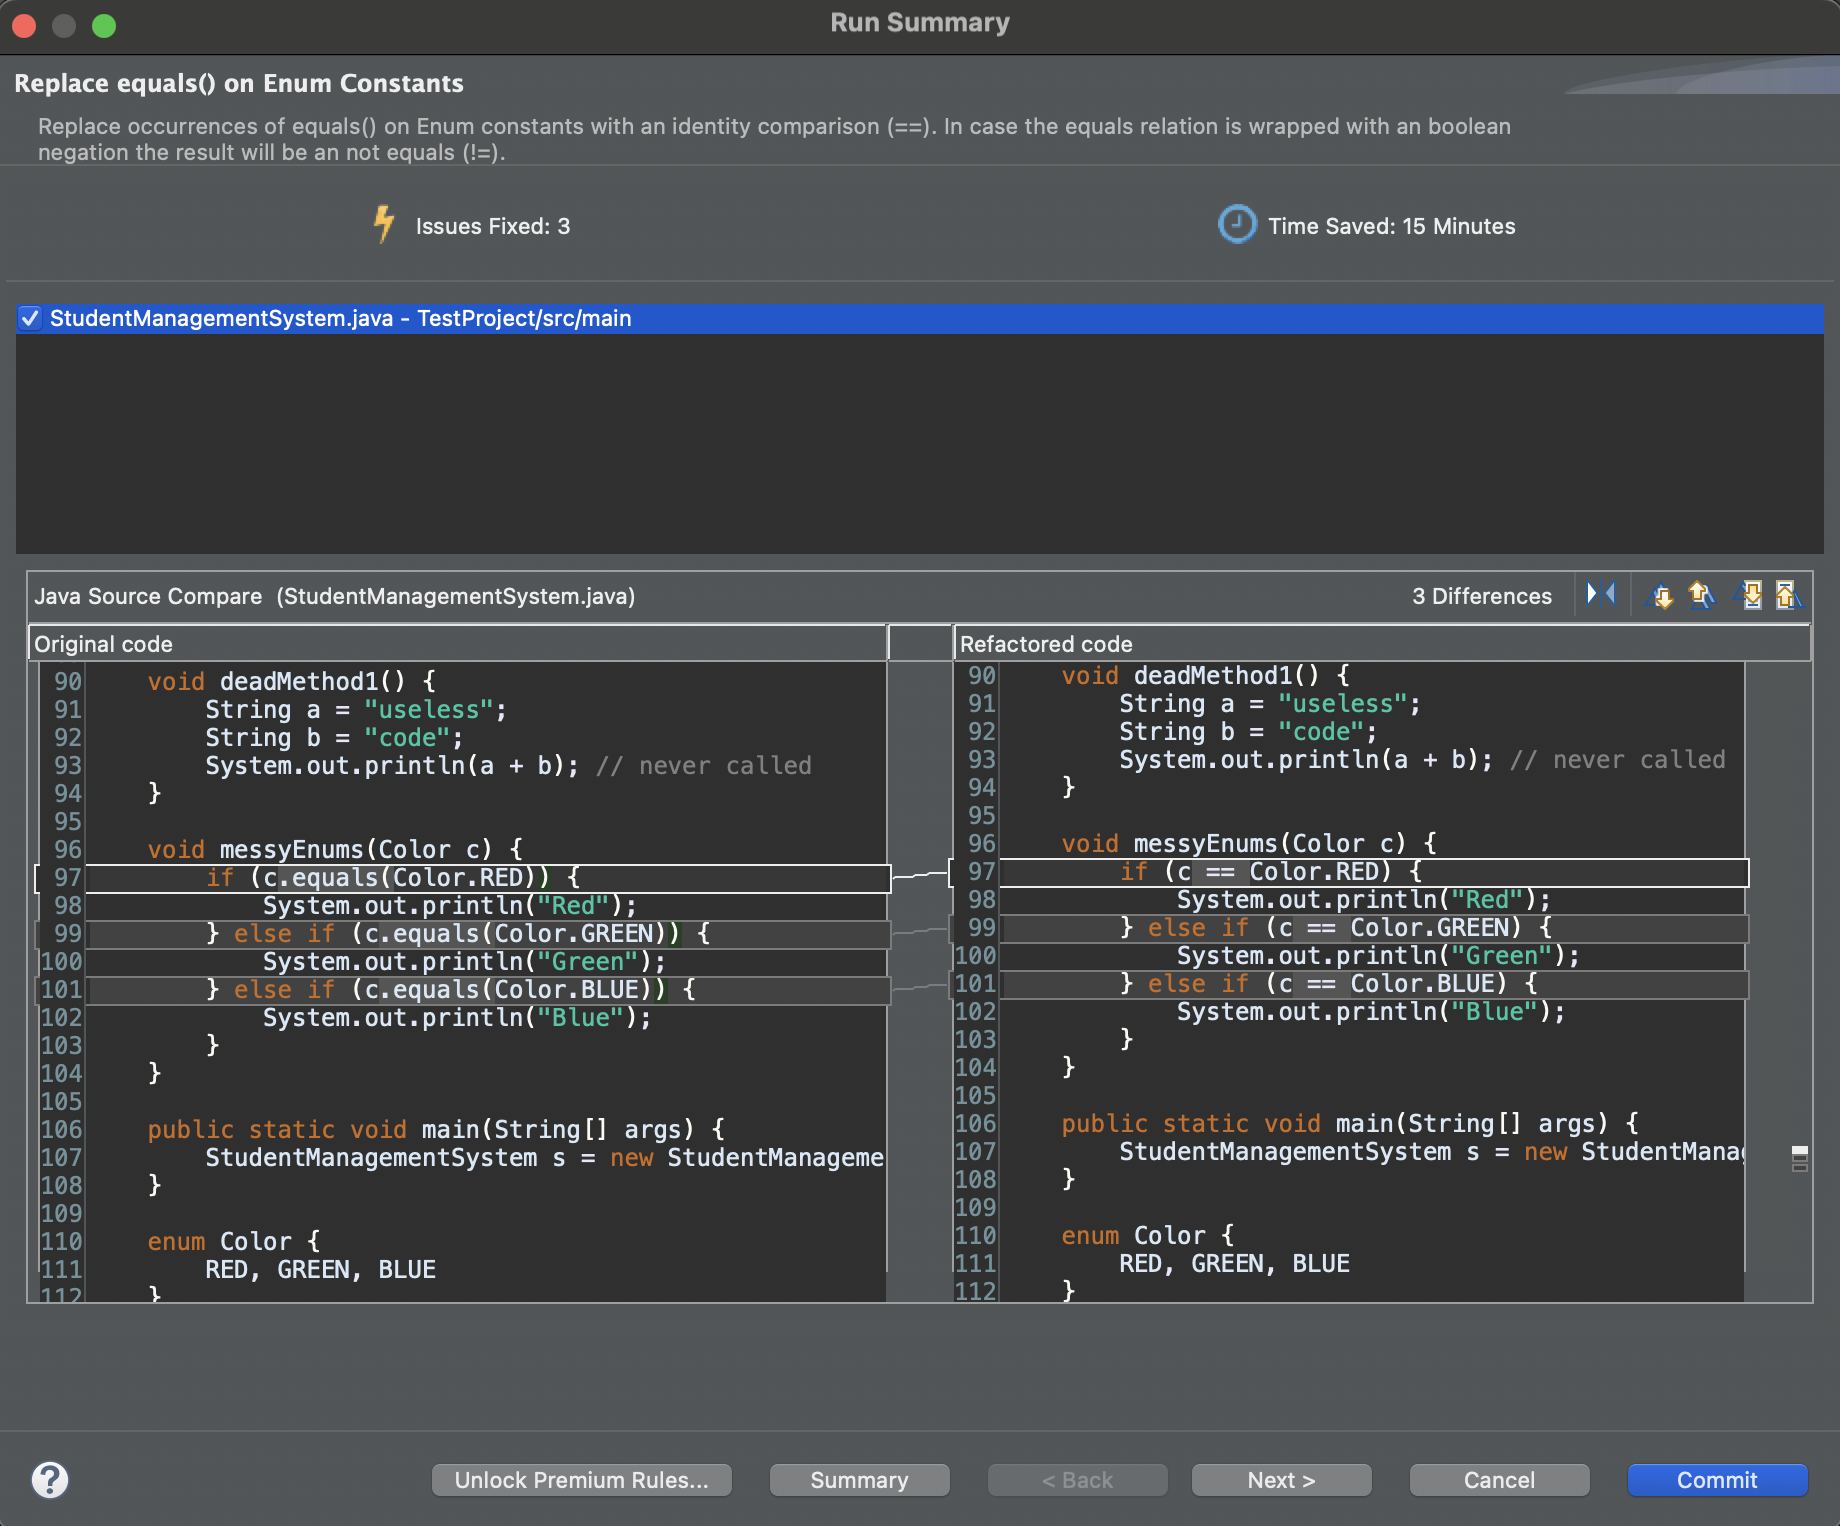
\includegraphics[width=0.5\textwidth]{issue-1-3.png}
  \caption{Replacement of equals() with == for Enum Constants}
  \label{fig:issue-1-3}
\end{figure}

\textbf{Rule: Replace equals() on Enum Constants.} This transformation replaced the use of \texttt{.equals()} with \texttt{==} when comparing enum constants. Since enums are singleton instances in Java, using \texttt{==} is both safe and more performant. This change improves both clarity and efficiency.

\begin{figure}[H]
  \centering
  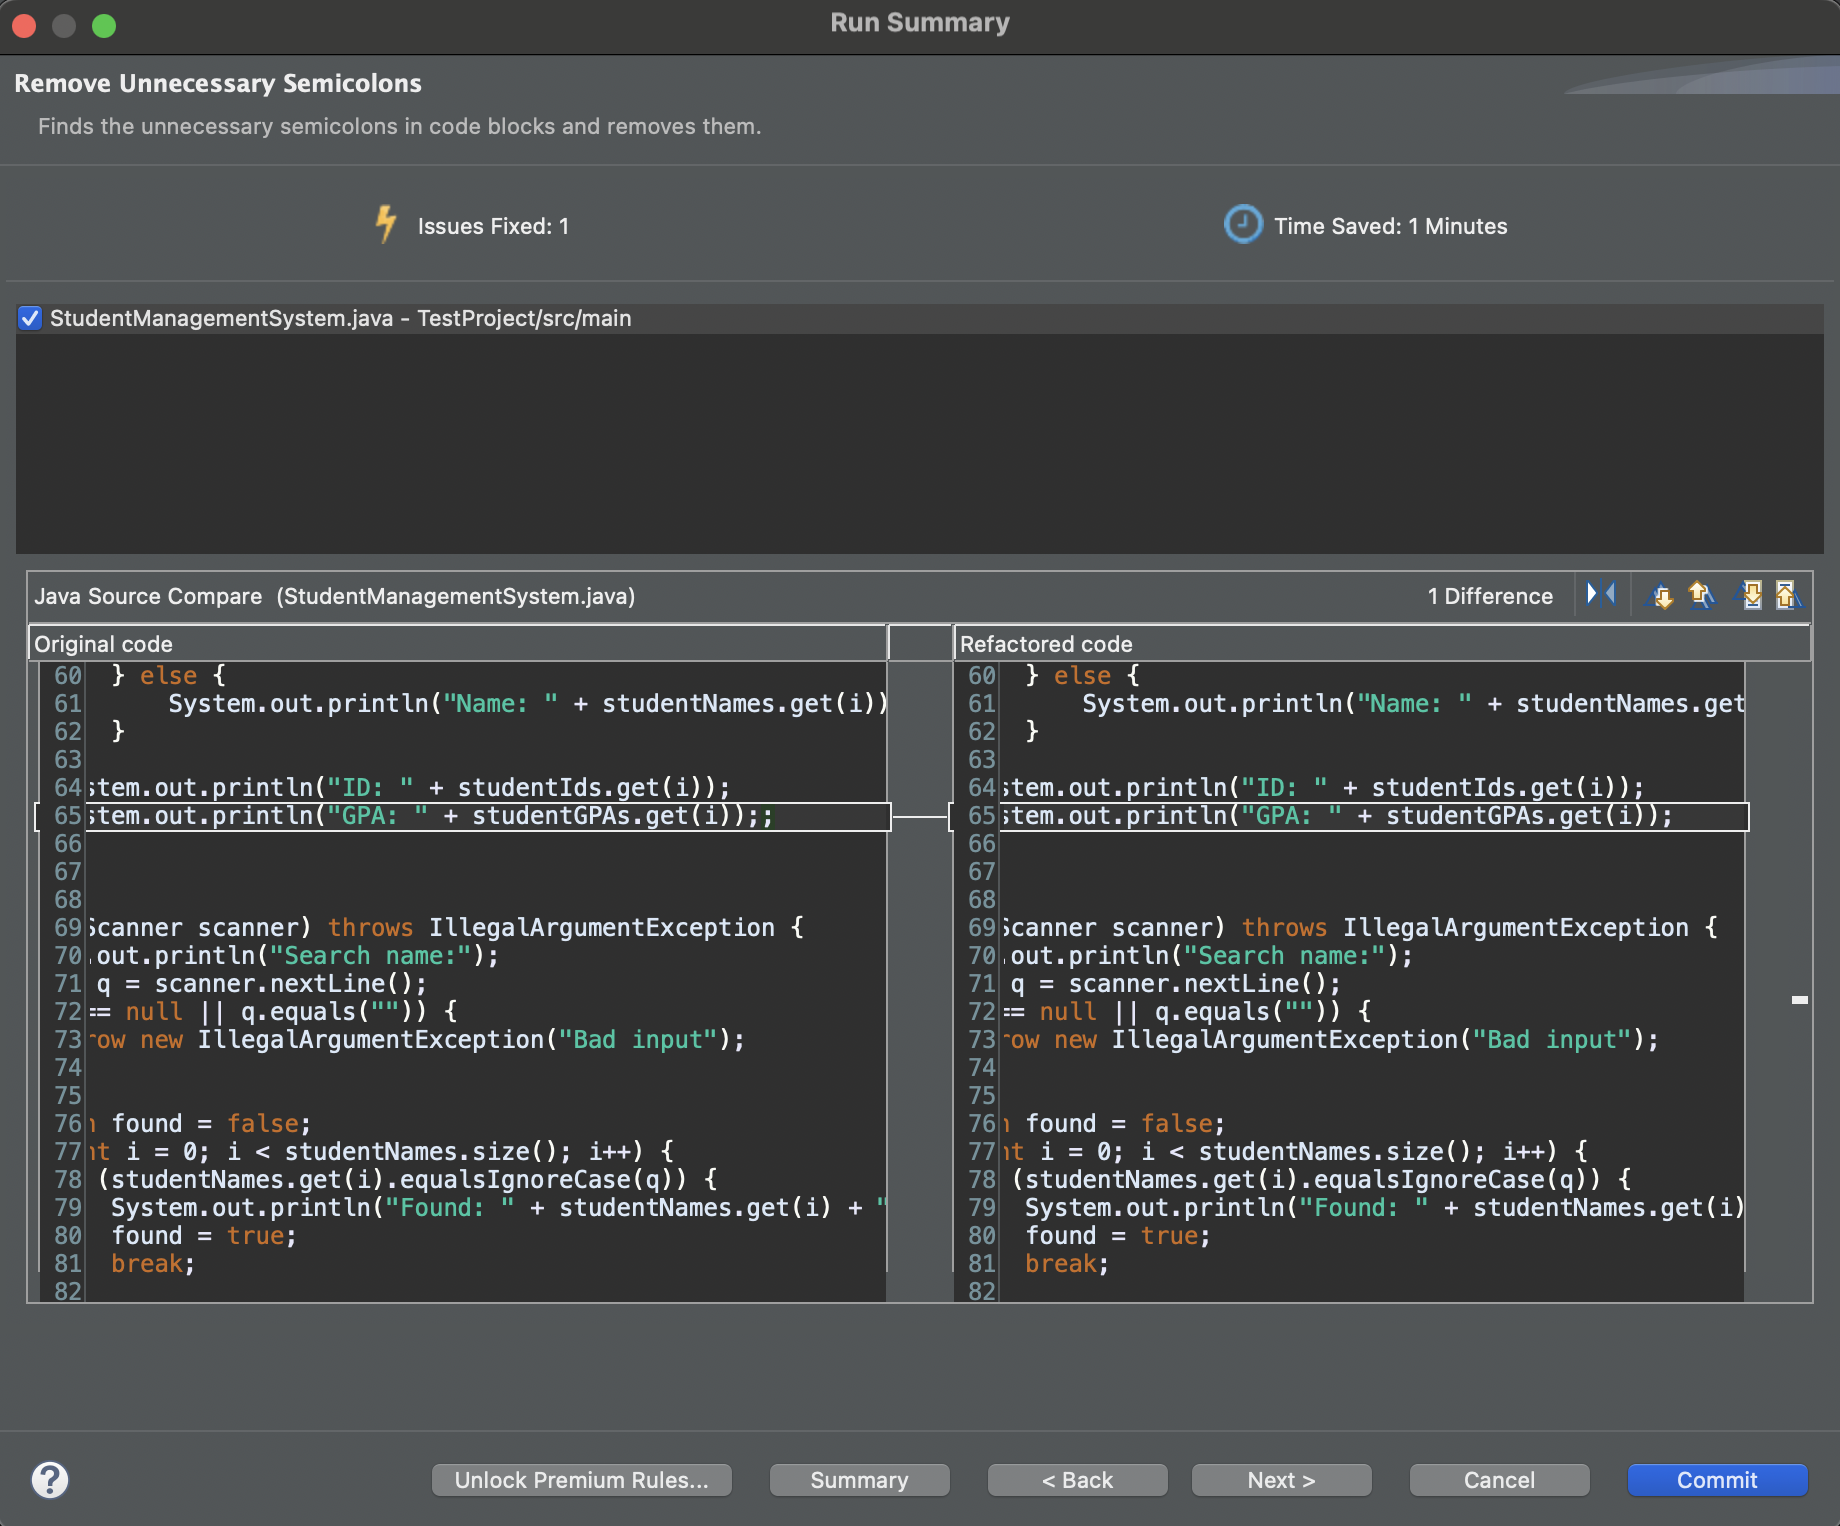
\includegraphics[width=0.5\textwidth]{issue-4.png}
  \caption{Remove Unnecessary Semicolons}
  \label{fig:issue-4}
\end{figure}

\textbf{Rule: Remove Unnecessary Semicolons.} In this figure, jSparrow successfully removed a dangling semicolon after a method call. However, the tool failed to detect multiple semicolons on the same line in this statement:
\texttt{ArrayList<String> studentNames = new ArrayList<>(); ArrayList<Integer> studentIds = new ArrayList<>(); ArrayList<Double> studentGPAs = new ArrayList<>();;} — showing a limitation in multi-statement detection.

\begin{figure}[H]
  \centering
  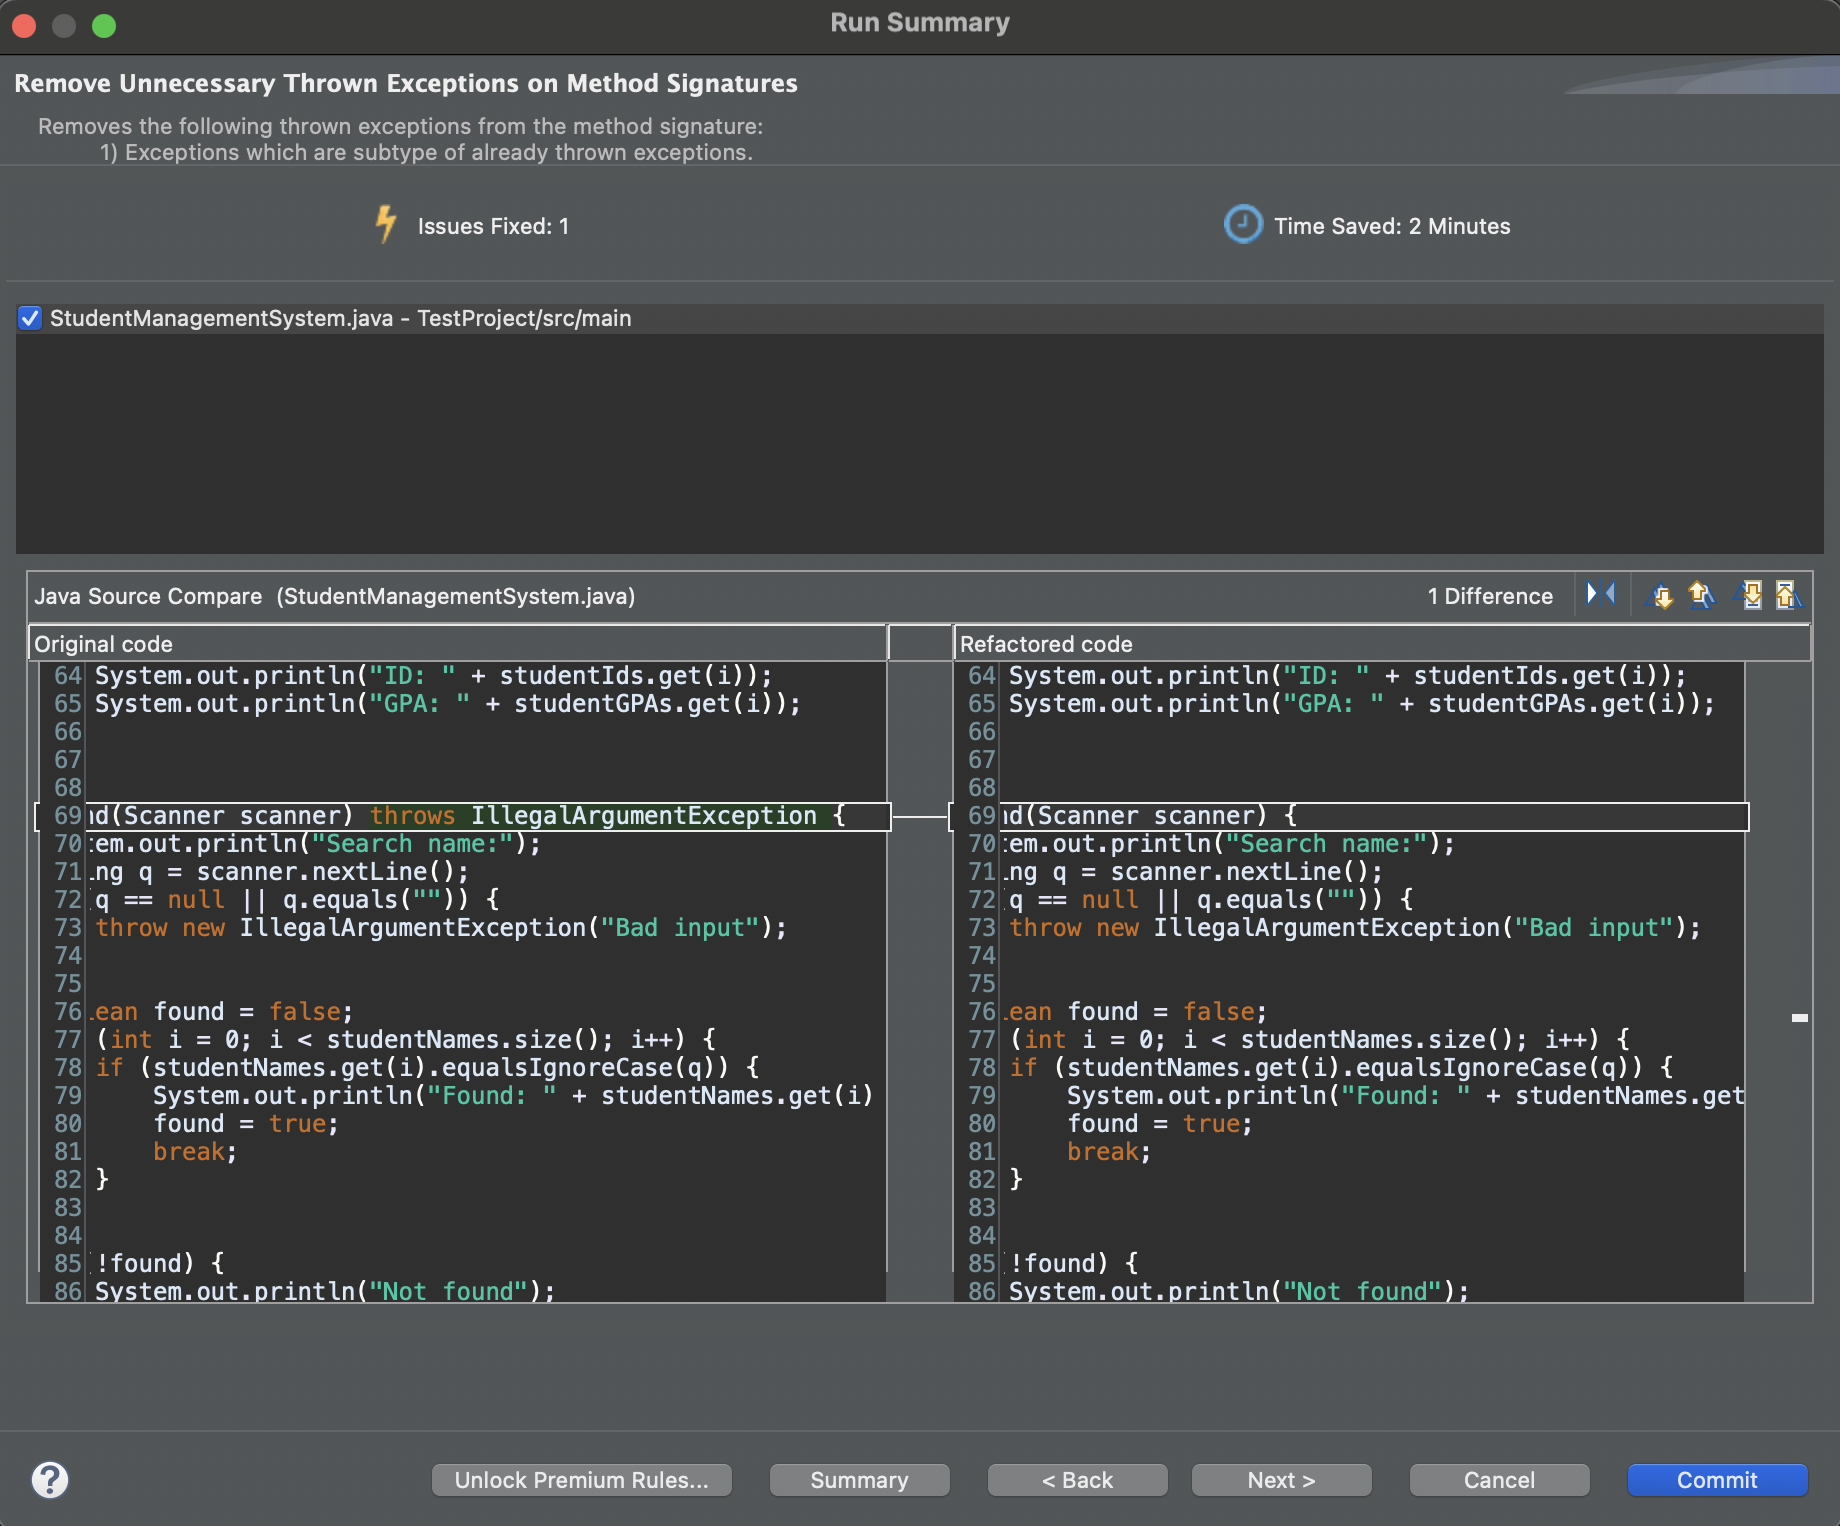
\includegraphics[width=0.5\textwidth]{issue-5.png}
  \caption{Remove Unnecessary Thrown Exceptions}
  \label{fig:issue-5}
\end{figure}

\textbf{Rule: Remove Unnecessary Thrown Exceptions on Method Signatures.} The \texttt{throws IllegalArgumentException} clause was removed from the method signature. This is safe and improves cleanliness because the exception is unchecked and does not need to be declared. The method behavior remains unchanged.

\begin{figure}[H]
  \centering
  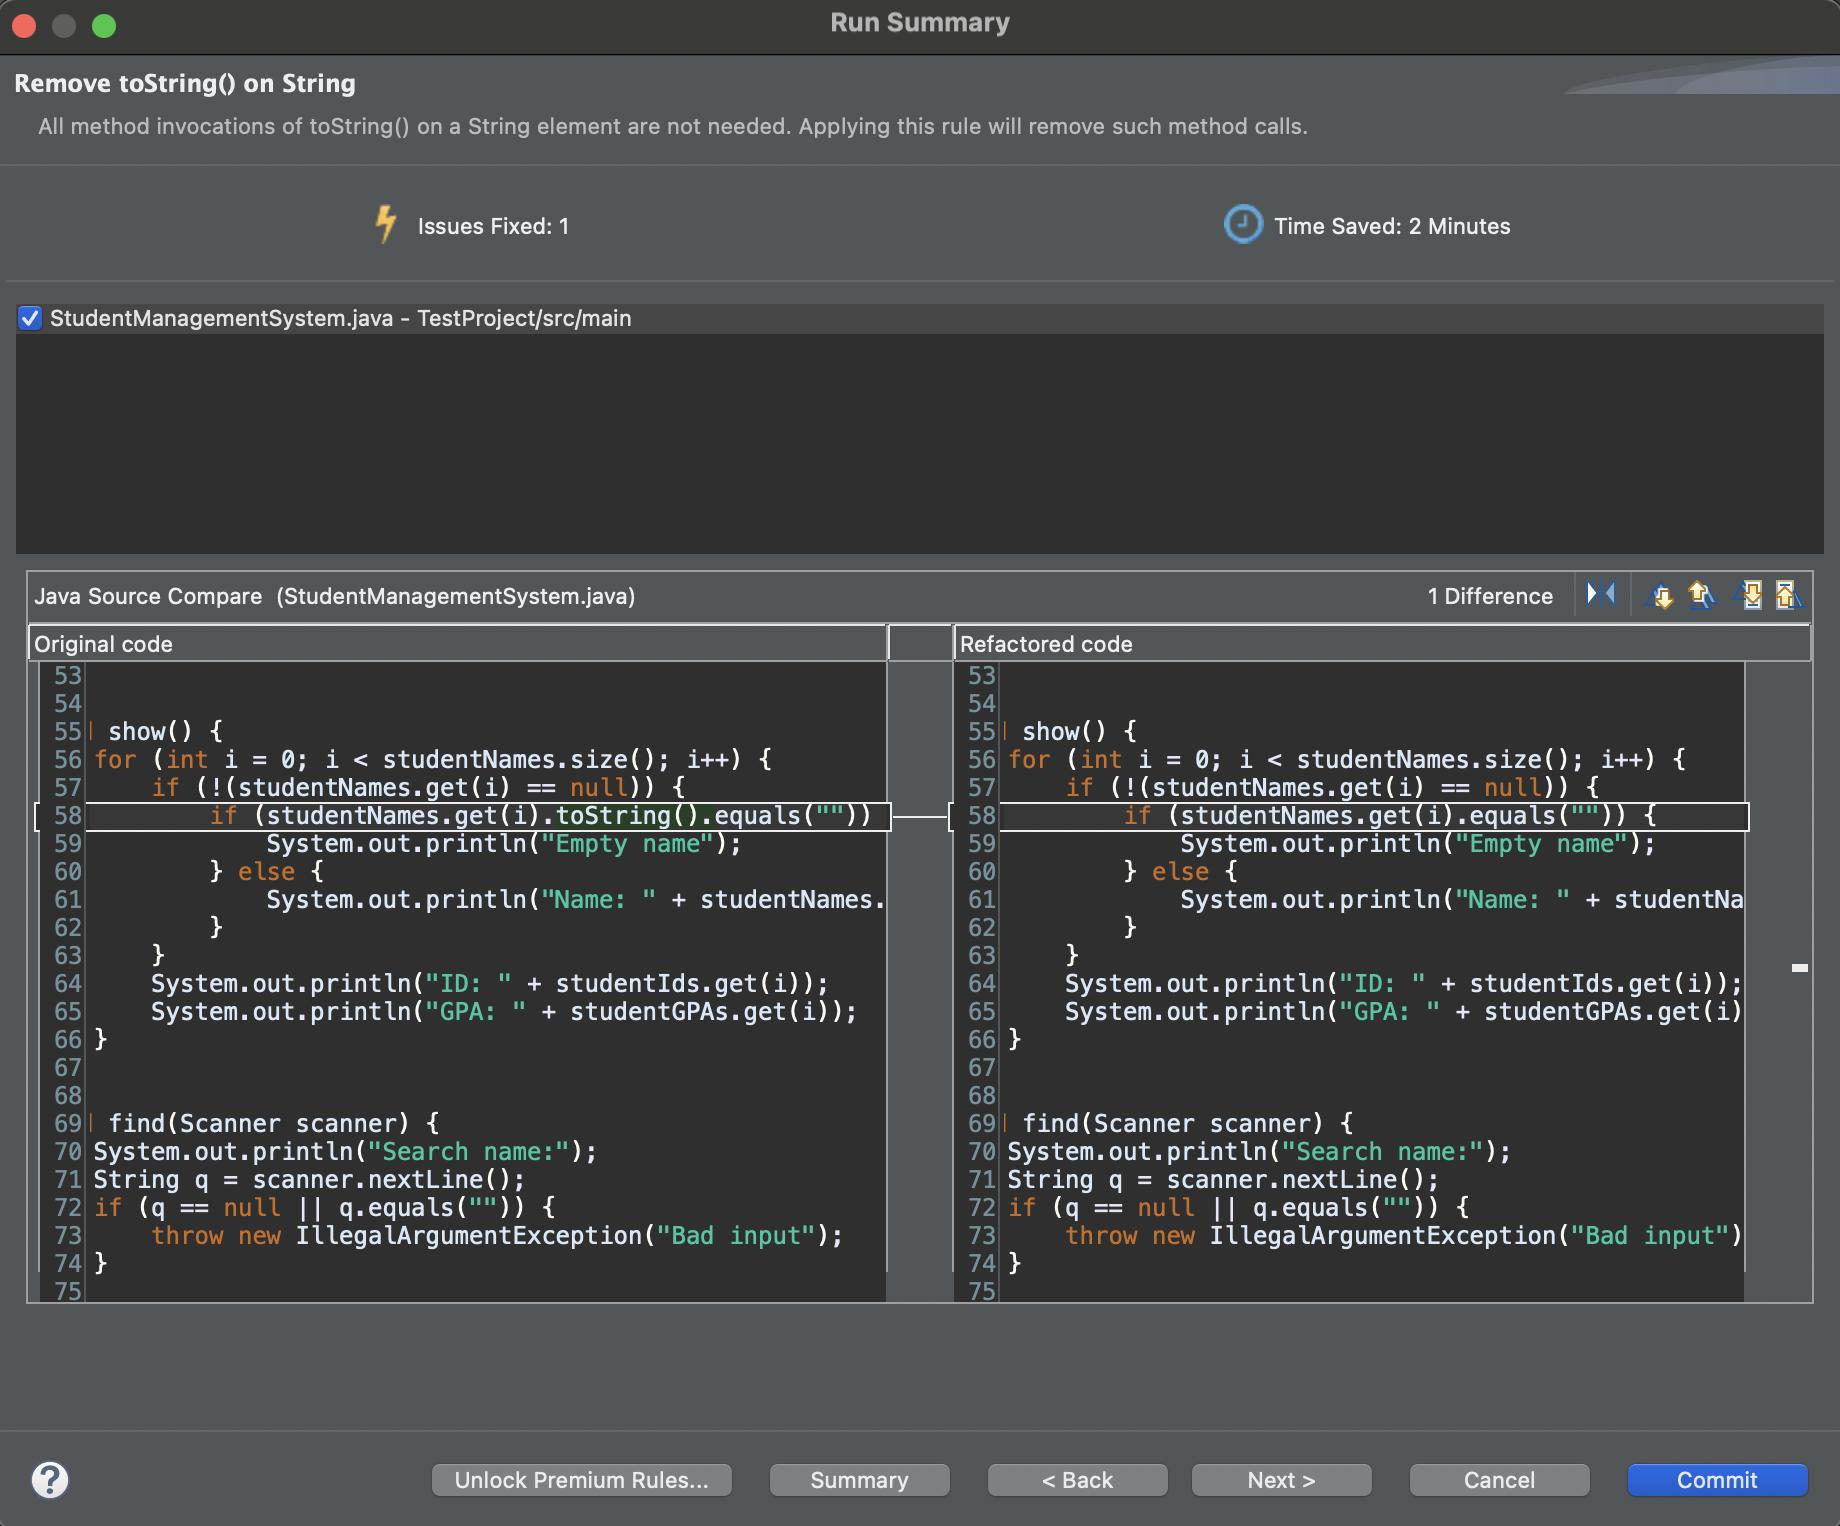
\includegraphics[width=0.5\textwidth]{issue-6.png}
  \caption{Remove toString() on String}
  \label{fig:issue-6}
\end{figure}

\textbf{Rule: Remove toString() on String.} The tool identified a redundant \texttt{toString()} call on a String instance. Since \texttt{studentNames.get(i)} already returns a String, the call was unnecessary. Removing it avoids clutter and improves clarity.

\begin{figure}[H]
  \centering
  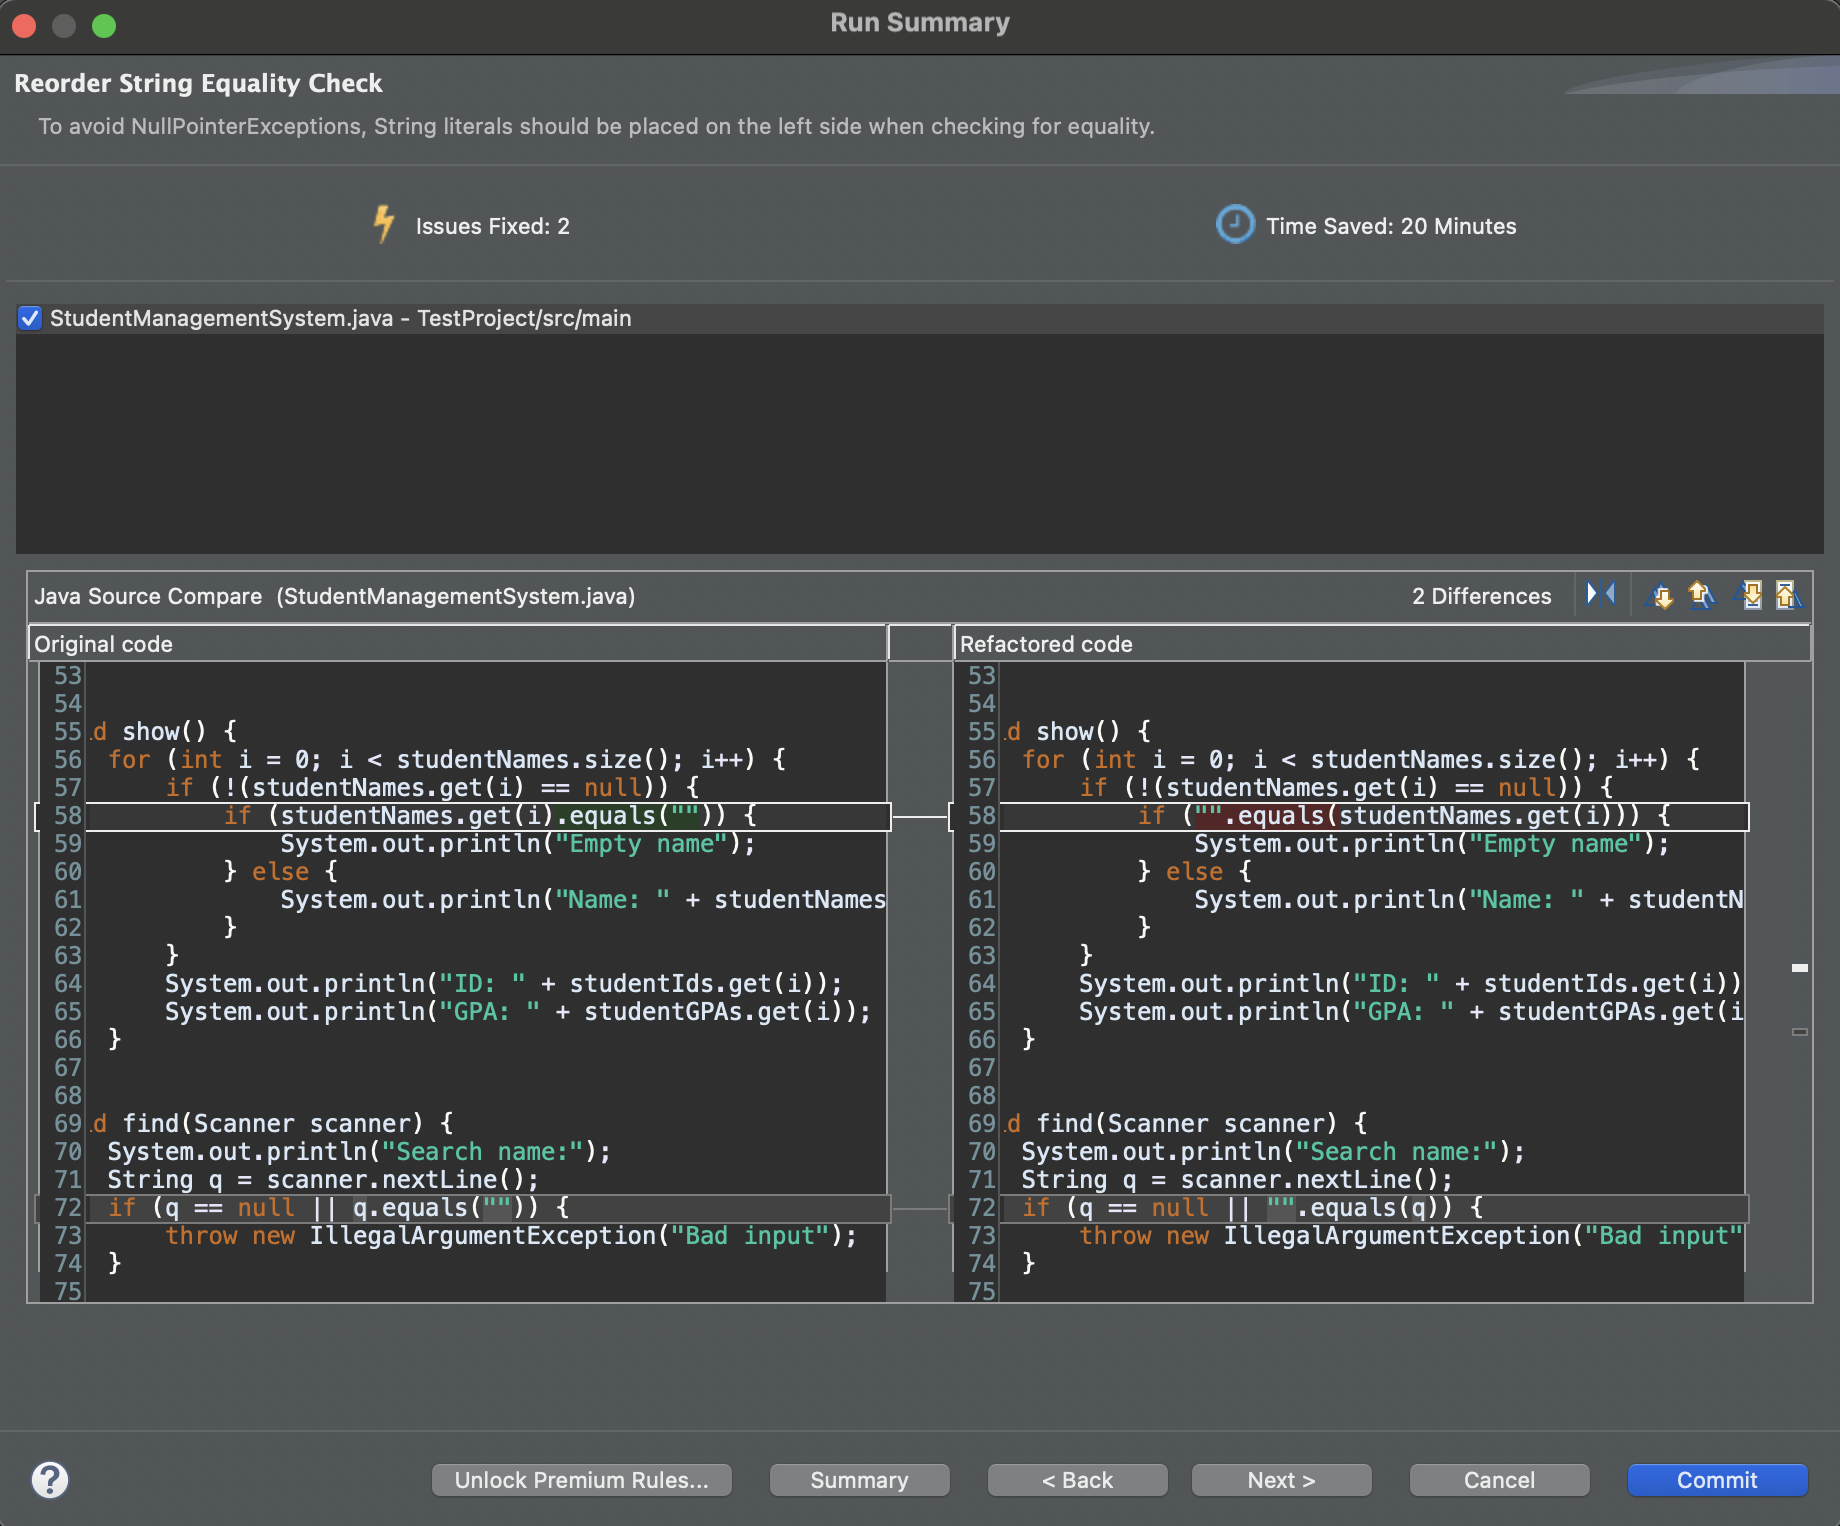
\includegraphics[width=0.5\textwidth]{issue-7-8.png}
  \caption{Reorder String Equality Checks}
  \label{fig:issue-7-8}
\end{figure}

\textbf{Rule: Reorder String Equality Checks.} jSparrow rearranged \texttt{variable.equals("")} into \texttt{"".equals(variable)} to prevent potential \texttt{NullPointerException}s when the variable is null. This is a common best practice in Java, particularly when working with user input or external data. The tool correctly applied this fix to multiple locations in the code.

\begin{figure}[H]
  \centering
  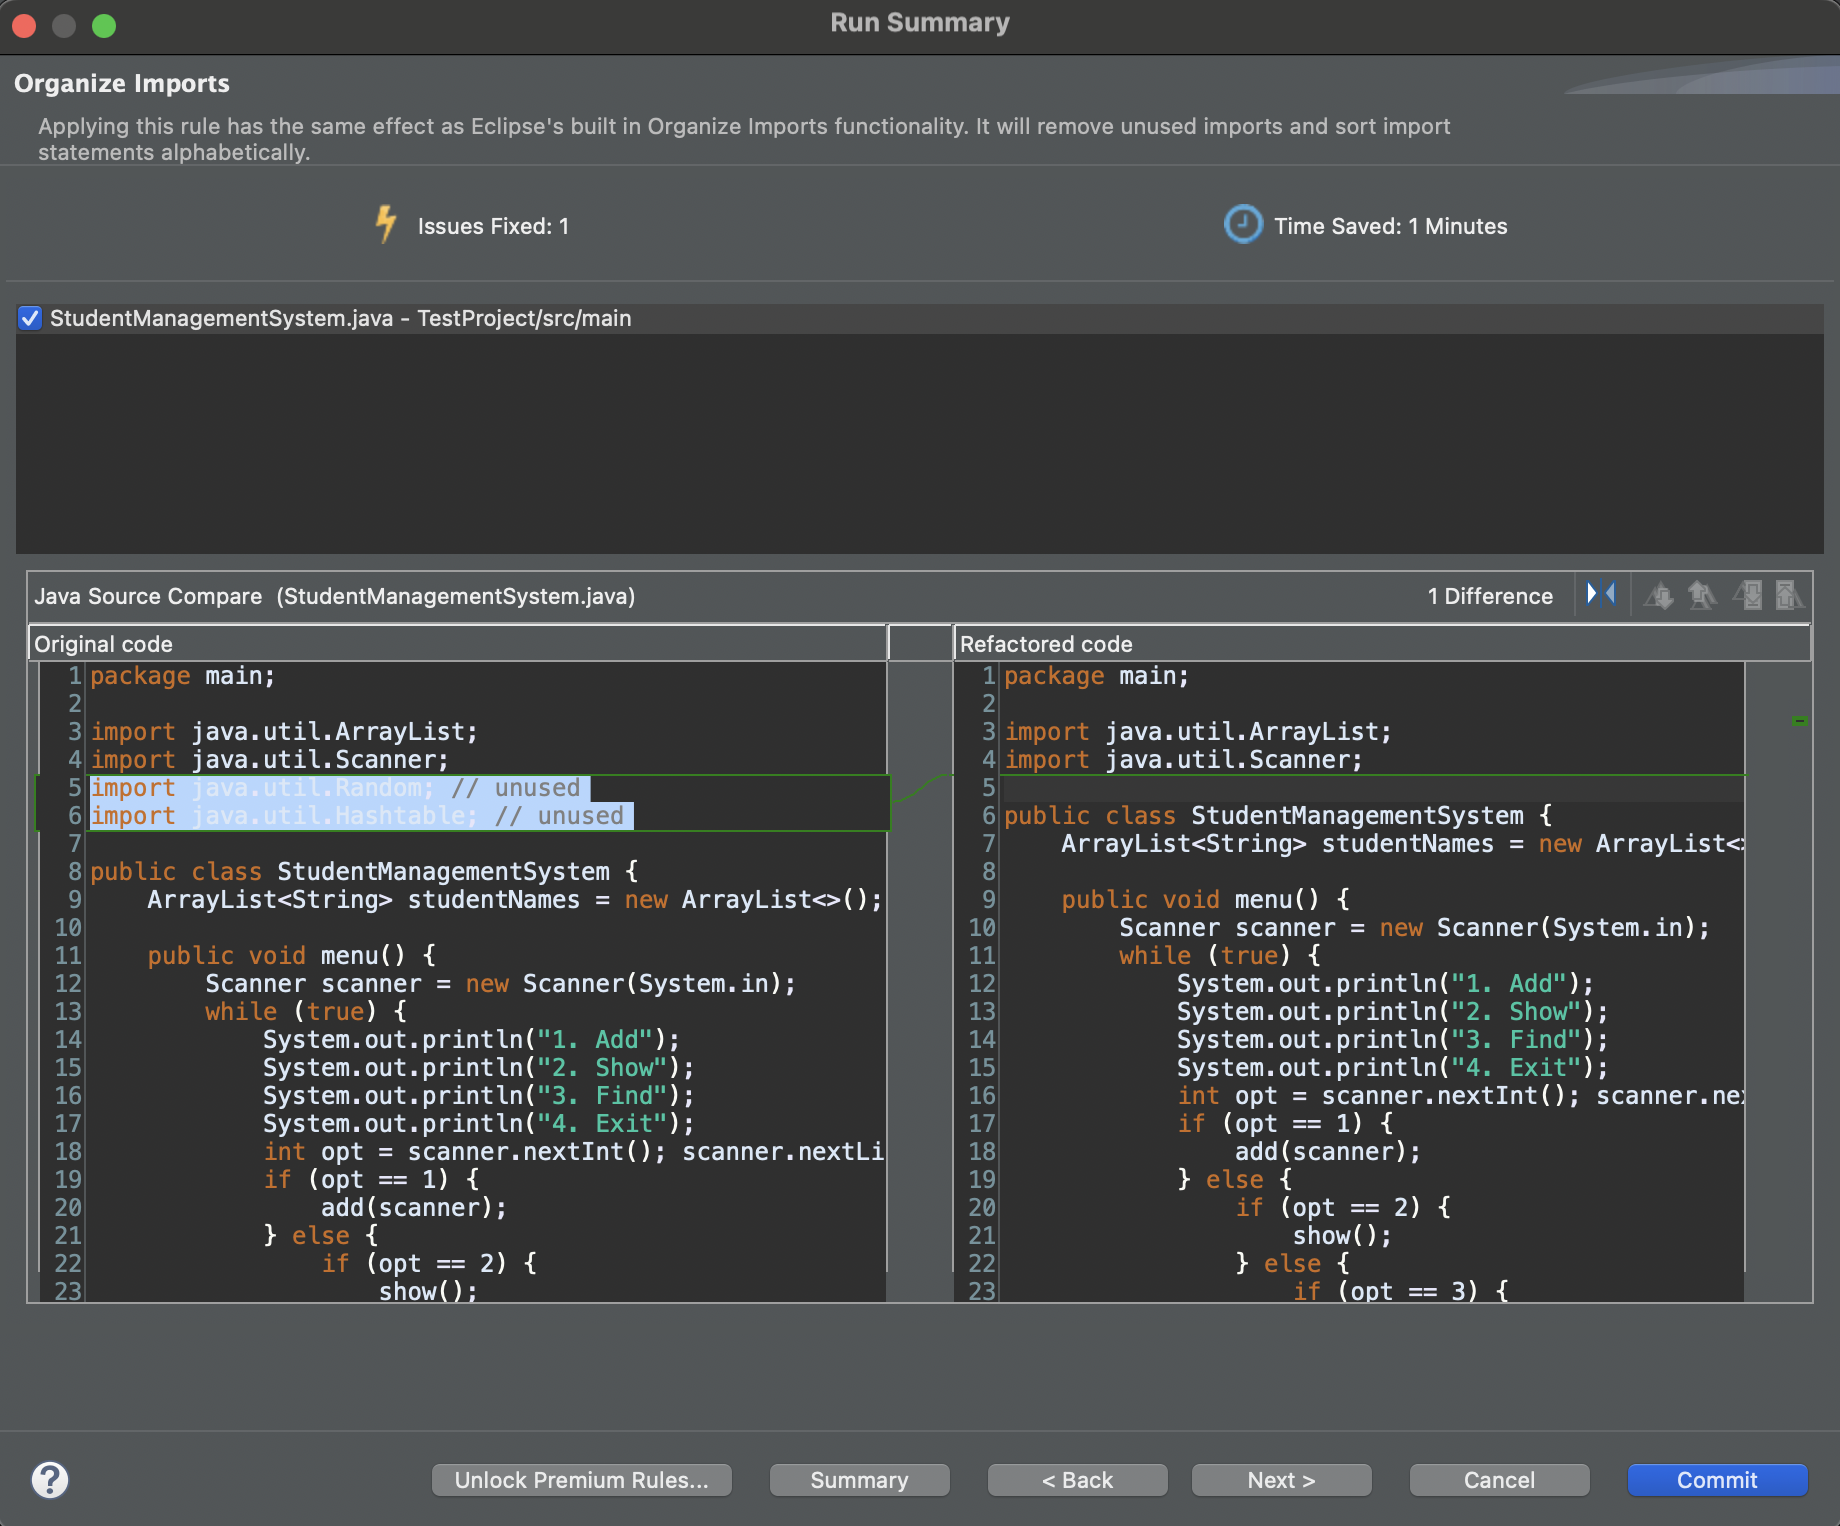
\includegraphics[width=0.5\textwidth]{issue-9.png}
  \caption{Organize Imports – Remove Unused Imports}
  \label{fig:issue-9}
\end{figure}

\textbf{Rule: Organize Imports.} Unused imports for \texttt{Random} and \texttt{Hashtable} were removed. This reduces code size and avoids misleading developers into thinking those classes are used. The remaining imports were sorted alphabetically, improving readability and adherence to conventions.

\begin{figure}[H]
  \centering
  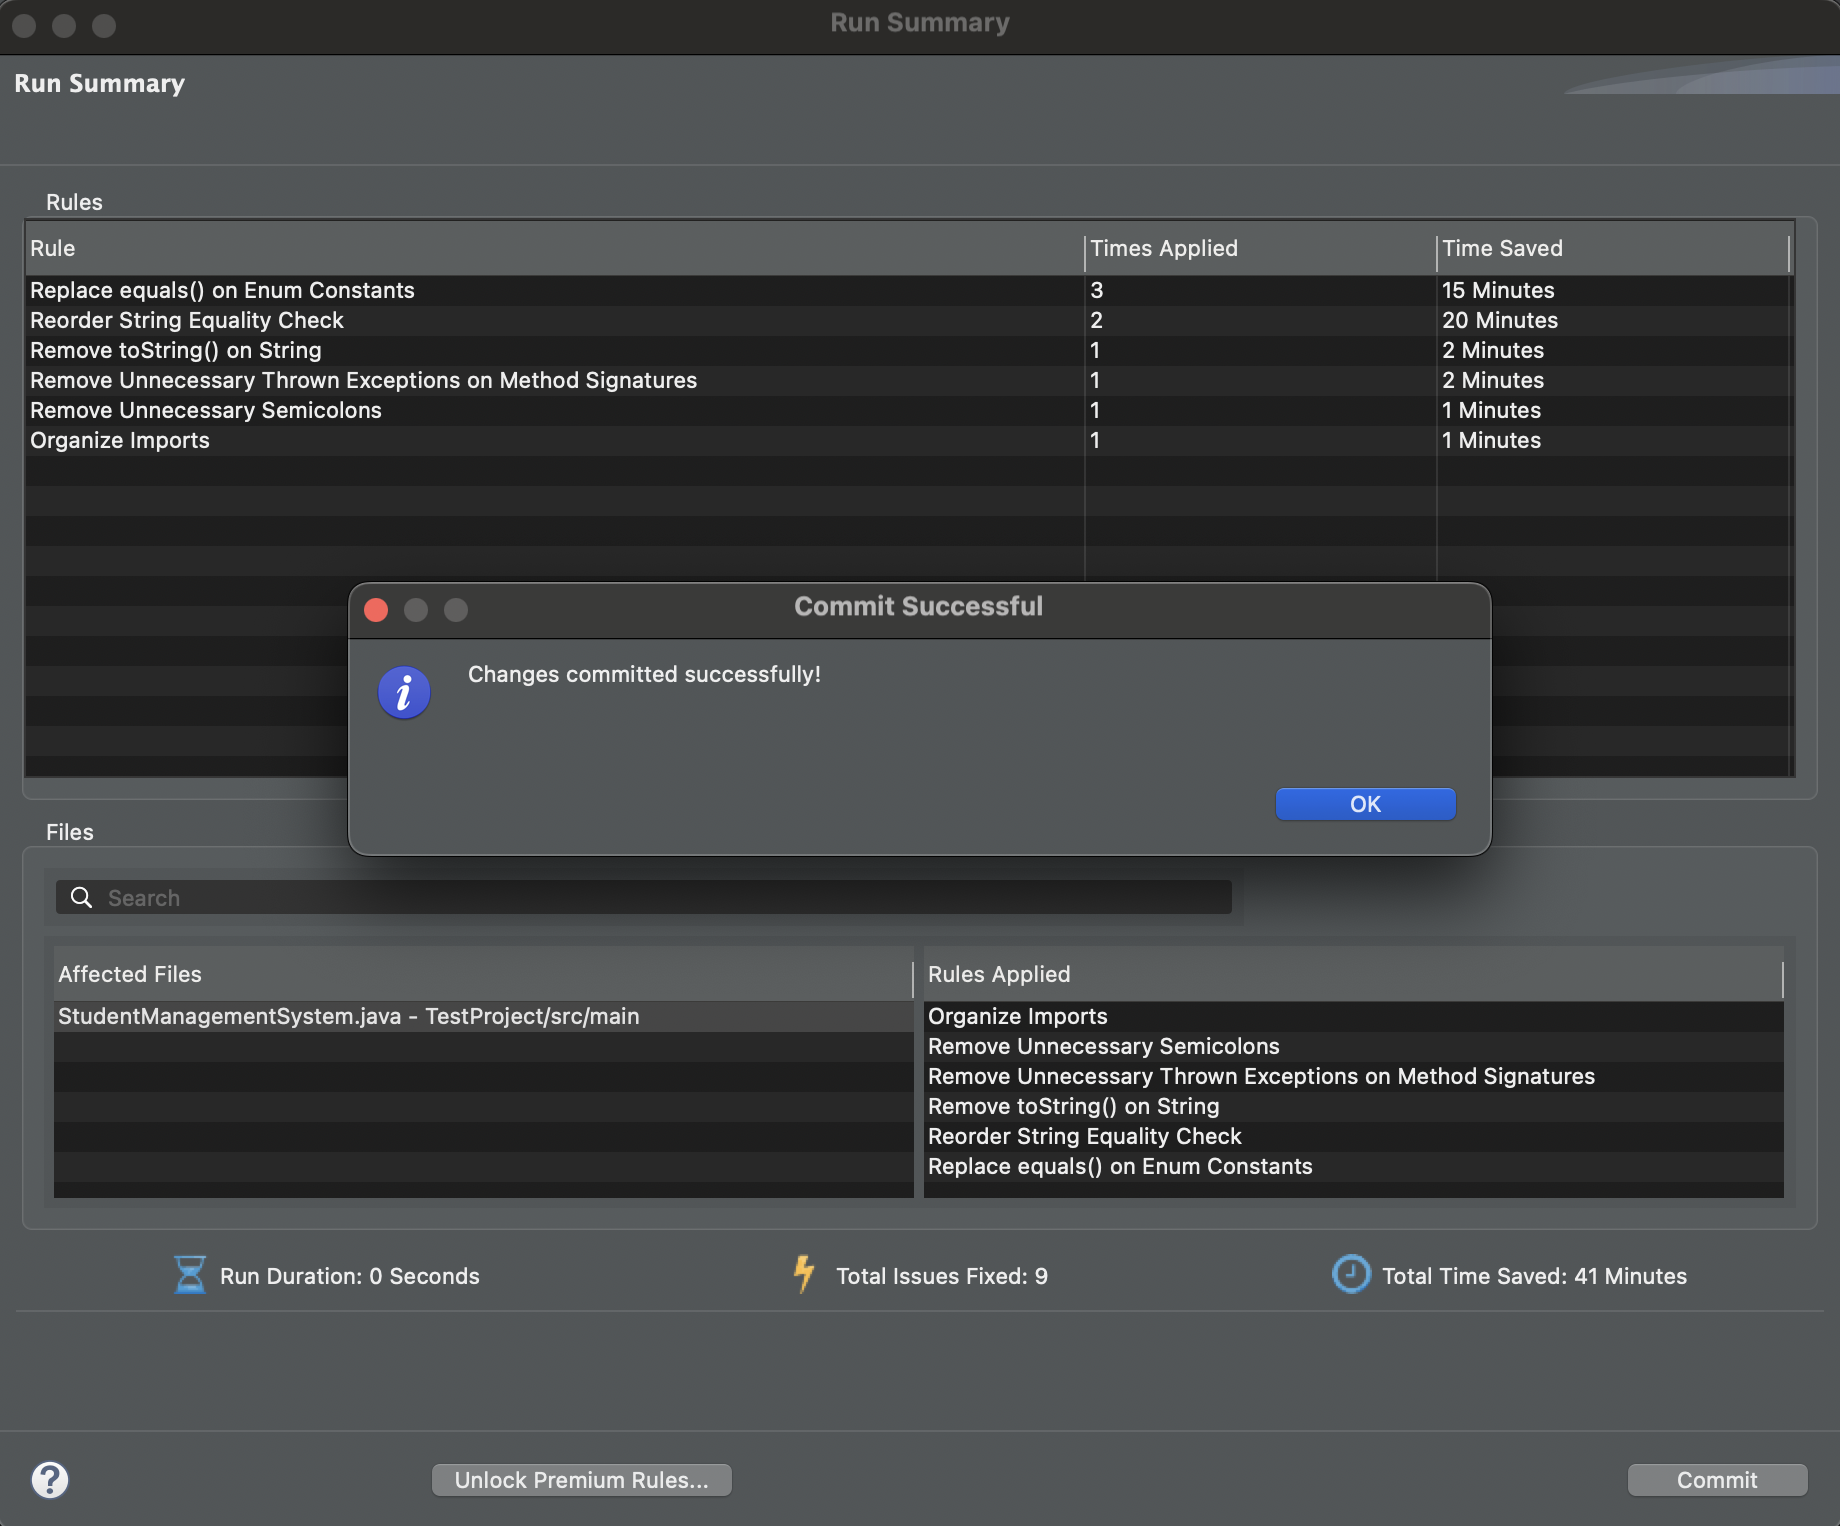
\includegraphics[width=0.5\textwidth]{commit-changes.png}
  \caption{Commit Summary by jSparrow}
  \label{fig:commit-changes}
\end{figure}

\textbf{Summary of Refactorings.} As seen in Figure~\ref{fig:commit-changes}, a total of 9 issues were fixed with an estimated time saving of 41 minutes. All fixes were applied to a single file. The commit window confirms that each rule was applied consistently, and the tool grouped the changes logically to allow review before committing.

\section{Conclusion}

As shown in Figure~\ref{fig:commit-changes}, jSparrow reported 9 issues fixed, saving an estimated 41 minutes. While it successfully handled several critical refactorings like enum comparison, import cleanup, and redundant operations, it missed some nuanced cases like multiple statements on a single line with excessive semicolons. Nonetheless, for a free tool, it provides valuable assistance in applying consistent code transformations and improving maintainability. The interface is user-friendly, allowing preview and confirmation before applying changes.

\end{document}
